% !TeX program = xelatex
% !TeX options = -shell-escape
% !TEX encoding = UTF-8

% --------------------------------------------------------------
% This is all preamble stuff that you don't have to worry about.
% Head down to where it says "Start here"
% --------------------------------------------------------------

\documentclass[12pt]{article}
\usepackage[margin=2cm]{geometry} % 頁面邊距設置
\usepackage{amsmath,amssymb,amsthm} % 數學相關套件
\usepackage{graphicx} % 圖形插入
\usepackage{booktabs} % 表格線條
\usepackage[AutoFakeBold,AutoFakeSlant]{xeCJK} % 中文支援
\usepackage{fancyhdr} % 頁首頁尾設置
\usepackage{xcolor,changepage,mdframed} % 顏色與框線相關
\usepackage{titlesec} % 標題格式
\usepackage{setspace} % 行距
\usepackage{minted} % 程式碼高亮（需安裝 Python 套件 pygments）
\usepackage[shortlabels]{enumitem} % 列表格式
\usepackage[colorlinks=true,linkcolor=black,urlcolor=blue,citecolor=blue]{hyperref}
% 超連結
\graphicspath{{images}}

% 字體設定 (xeCJK)
\setCJKmainfont{黑體-繁}
\setCJKmonofont{Noto Sans CJK TC}

% 頁首/頁尾設定 (fancyhdr)
\pagestyle{fancy}
\fancyhead[L]{NASA Homework 6} % 可以用 \leftmark 取代
\fancyhead[R]{B13901011 吳亞倫}
\fancyfoot[C]{\thepage}
\renewcommand{\headrulewidth}{0.4pt}
\renewcommand{\footrulewidth}{0pt}
\setlength{\headheight}{15pt}

% tex-fmt: off
\newtheorem*{theorem}{Theorem}
\newenvironment{lemma}[2][Lemma]{\begin{trivlist}
\item[\hskip \labelsep {\bfseries #1}\hskip \labelsep {\bfseries #2.}]}{\end{trivlist}}
\newenvironment{exercise}[2][Exercise]{\begin{trivlist}
\item[\hskip \labelsep {\bfseries #1}\hskip \labelsep {\bfseries #2.}]}{\end{trivlist}}
\newenvironment{problem}[2][Problem]{\begin{trivlist}
\item[\hskip \labelsep {\bfseries #1}\hskip \labelsep {\bfseries #2}]}{\end{trivlist}}
\newenvironment{question}[2][Question]{\begin{trivlist}
\item[\hskip \labelsep {\bfseries #1}\hskip \labelsep {\bfseries #2.}]}{\end{trivlist}}
\newenvironment{corollary}[2][Corollary]{\begin{trivlist}
\item[\hskip \labelsep {\bfseries #1}\hskip \labelsep {\bfseries #2.}]}{\end{trivlist}}
\newenvironment{solution}{\begin{proof}[Solution]}{\end{proof}}
\newenvironment{answer}{\begin{proof}[Ans]}{\end{proof}}

% 樣式設定

\setminted{frame=lines, linenos, framesep=2mm, breaklines=true, breakanywhere=true, autogobble=true}

% 自訂框線環境
\newmdenv[
  linewidth=2pt, linecolor=gray, backgroundcolor=gray!10,
  topline=false, bottomline=false, rightline=false,
  skipabove=10pt, skipbelow=10pt, innerleftmargin=10pt,
  innerrightmargin=0pt, innertopmargin=5pt, innerbottommargin=5pt
]{myquote}

\newenvironment{mycolorbox}[1][gray]{
  \renewmdenv[
    linewidth=2pt, linecolor=#1, backgroundcolor=#1!10,
    topline=false, bottomline=false, rightline=false,
    skipabove=10pt, skipbelow=10pt, innerleftmargin=10pt,
    innerrightmargin=0pt, innertopmargin=5pt, innerbottommargin=5pt
  ]{myquote}
  \begin{myquote}
}{\end{myquote}}

\linespread{1.1}
% \usemintedstyle{xcode}
\AtBeginEnvironment{minted}{\vspace{-10pt}} % 可根據需求調整間距數值
\setminted{breaklines=true, breakanywhere=true, autogobble=true}

% tex-fmt: on
\begin{document}
\thispagestyle{fancy}

%------------------------------------------------------------
%                         Start here
% -----------------------------------------------------------

\begin{center}
  {\large \bfseries Network Administration / System Administration} \\
  \vspace{1em}
  {\Large \bfseries Homework 7} \\
\end{center}

\vspace{2em}

\begin{tabular}{@{}l l}
  \textbf{Student:} & 吳亞倫 \\
  \textbf{ID:} & B13901011  \\
  \textbf{Department:} & 電機工程學系
\end{tabular}
\bigskip

\begin{mycolorbox}[cyan]
  \textbf{Discussion Partners:}
  \begin{itemize}
    \item Classmates：賴泓安、鄭竣陽、喻慈恩
      \vspace{0.5em}
  \end{itemize}
\end{mycolorbox}

% -----------------------------------------------------------
% Problem 1
% -----------------------------------------------------------
\section{PVE}
\begin{mycolorbox}[teal]
  \textbf{Reference:} 
  \footnotesize
  \begin{itemize}
    \item \url{https://linux.vbird.org/linux_server/rocky9/0130vmtuning.php}
    \item \url{https://linux.die.net/man/1/virt-install}
    \item \href{https://blog.gtwang.org/linux/kvm-qemu-virt-install-command-tutorial/}{KVM/QEMU 以 virt-install 指令建立虛擬機器、VNC 顯示畫面教學}
    \item \url{https://johnliu55.tw/ssh-tunnel.html}
  \end{itemize}
\end{mycolorbox}


% Problem 1.1
\subsection{}
\begin{enumerate}
  \item 透過以下指令建立 qcow2 硬碟：
  \begin{minted}{bash}
    qemu-img create -f qcow2 /tmp2/b13901011/hw7/pve1.qcow2 10G
  \end{minted}

  \item 透過以下指令安裝虛擬機：
  \begin{minted}{bash}
    virt-install --virt-type kvm \
      --name b13901011-1 \
      --vcpu 2 \
      --memory 8192 \
      --os-variant generic \
      --cdrom /tmp2/rabhunter/hw7/proxmox.iso \
      --disk path=/tmp2/b13901011/hw7/pve1.qcow2,format=qcow2 \
      --network bridge=br0,mac=52:54:90:10:11:01 \
      --graphics vnc,port=7000,listen=0.0.0.0,password=nasa2025 \
      --noautoconsole
  \end{minted}

  \item 以 vnc 連線上去後，點 graphics install。以下為我安裝的虛擬機器的設定：
  \begin{figure}[H]
    \centering
    
\includegraphics[width=0.9\textwidth]{1-1-2.png}
    \caption{虛擬機器設定}
    \label{fig:1-1-2}
  \end{figure}
  \item 安裝完成後，透過以下指令啟動虛擬機器：
  \begin{minted}{bash}
    virsh start b13901011-1
  \end{minted}
  並且以 vnc 連線上虛擬機，獲得以下畫面：
  \begin{figure}[H]
    \centering
    
\includegraphics[width=0.8\textwidth]{1-1-3.png}
    \caption{虛擬機器啟動畫面}
    \label{fig:1-1-3}
  \end{figure}

\end{enumerate}


% Problem 1.2
\subsection{}
在 pve1 上，我使用 \texttt{ip r} 得知 ip 位置為 \texttt{192.168.128.225}，並在工作站上 \texttt{ping} 和 \texttt{ssh} 成功。
\begin{figure}[H]
  \centering
  
\includegraphics[width=0.8\textwidth]{1-2-1.png}
  \caption{ping 192.168.128.225 成功}
  \label{fig:1-2-1}
\end{figure}

% Problem 1.3
\subsection{}
\begin{enumerate}
  \item 在我電腦本地端，我使用以下指令建立 ssh tunnel：
  \begin{minted}{bash}
    ssh -L 8006:192.168.128.225:8006 b13901011@nasaws1.csie.ntu.edu.tw
  \end{minted}
  \item 在本地端的瀏覽器上輸入 \texttt{localhost:8006}，並且登入：
  \begin{figure}[H]
    \centering
    
\includegraphics[width=\textwidth]{1-3-1.png}
    \caption{登入畫面}
    \label{fig:1-3-1}
  \end{figure}
\end{enumerate}

% -----------------------------------------------------------
% Problem 2
% -----------------------------------------------------------
\section{Create VM}
\begin{mycolorbox}[teal]
  \textbf{Reference:}
  \footnotesize
  \begin{itemize}
    \item \href{https://blog.csdn.net/cjj2006/article/details/134406290}{KVM給虛擬Linux加磁盤}
    \item \href{https://www.albert-yu.com/blog/proxmox-ve-%E5%88%9D%E5%A7%8B%E5%8C%96%E7%A1%AC%E7%A2%9F%E5%88%86%E5%89%B2%E5%8D%80%E8%88%87%E9%85%8D%E7%BD%AEzfs%E5%84%B2%E5%AD%98%E5%8D%80raidz/}{Proxmox VE 初始化硬碟分割區與配置ZFS儲存區}
    \item \href{https://libvirt.org/formatdomain.html#userspace-connection-using-slirp}{libvirt: Domain XML Format - Userspace Connection Using Slirp}
    \item \url{https://ithelp.ithome.com.tw/m/articles/10244708}
    \item \href{https://hk.unbxtech.com/2021/12/howto-create-vm-proxmox-ve-7.html}{如何在Proxmox VE 7中建立虛擬機器}
    \item \href{https://hackmd.io/@ict39/S1Orfipr_}{Alpine 安裝教學}
    \item \url{https://wiki.alpinelinux.org/wiki/Setting_up_a_new_user}
  \end{itemize}
\end{mycolorbox}

% Problem 2.1
\subsection{}
\begin{enumerate}
  \item 我使用以下指令建立 qcow2 硬碟，並且將它掛載到虛擬機器上：
  \begin{minted}{bash}
    qemu-img create -f qcow2 /tmp2/b13901011/hw7/pve1_2.qcow2 20G
    virsh attach-disk b13901011-1 /tmp2/b13901011/hw7/pve1_2.qcow2 vda --subdriver qcow2 --persistent
  \end{minted}
  \item 連線到 pve1 的 web UI 當中，點選 \texttt{b13901011-1}，然後點選 \texttt{disk} > \texttt{zfs} > \texttt{create zfs}，並且選擇 \texttt{vda}，然後點選 \texttt{create}。
  \begin{figure}[H]
    \centering
    
\includegraphics[width=0.8\textwidth]{2-1-1.png}
    \caption{建立 zfs}
    \label{fig:2-1-1}
  \end{figure}
\end{enumerate}

% Problem 2.2
\subsection{}
\begin{enumerate}
  \item 首先，我在工作站中，使用以下指令新增一個 interface：
  \begin{minted}{bash}
    virsh edit b13901011-1
  \end{minted}
  \item 接著，我在 \texttt{<devices>} 中新增一個 interface，並且將它的 mac 設定為 \texttt{52:54:90:10:11:02}，如下所示：
  \begin{minted}{xml}
    <interface type='user'>
        <mac address='52:54:90:10:11:02'/>
        <model type='virtio'/>
    </interface>
  \end{minted}
  \item 透過以下指令重新啟動虛擬機器：
  \begin{minted}{bash}
    virsh shutdown b13901011-1
    virsh start b13901011-1
  \end{minted}
  \item ssh 進去之後，我用 \texttt{ip a} 得知新增網卡位於 \texttt{ens7}，因此我編輯了 \texttt{/etc/network/interface}，並且新增設定如下：
  \begin{minted}{bash}
    auto ens7
    iface ens7 inet dhcp
        gateway 10.0.2.2
  \end{minted}
  \item 接著，我使用以下指令重新啟動網路：
  \begin{minted}{bash}
    systemctl restart networking
  \end{minted}
  \item 接者我修改 default gateway，如下所示：
  \begin{minted}{bash}
    ip route del default
    ip route add default via 10.0.2.2 dev ens7
  \end{minted}
  \item 最後，我使用以下指令檢查網路是否正常：
  \begin{minted}{bash}
    ip r
    ping google.com
  \end{minted}
  \begin{figure}[H]
    \centering
    
\includegraphics[width=0.8\textwidth]{2-2-1.png}
    \caption{ping google.com 成功}
    \label{fig:2-2-1}
  \end{figure}
\end{enumerate}


% Problem 2.3
\subsection{}

\begin{enumerate}
  \item 在 pve1 上，我編輯了 \texttt{/etc/network/interfaces}，並且新增設定如下：
  \begin{minted}{bash}
    auto ens7
    iface ens7 inet manual

    auto vmbr1
    iface vmbr1 inet manual
      address 10.0.2.15/24
      gateway 10.0.2.2
      bridge_ports ens7
      bridge_stp off
      bridge_fd 0
  \end{minted}
  \item 重新啟動網路服務：
  \begin{minted}{bash}
    ifreload -a
  \end{minted}
  \begin{figure}[H]
    \centering
    
\includegraphics[width=\textwidth]{2-3-1.png}
    \caption{橋接網路設定完成}
    \label{fig:2-3-1}
  \end{figure}
\end{enumerate}

% Problem 2.4
\subsection{}
\begin{enumerate}
  \item 首先，我從工作站中，將 alpine iso 檔案上傳到 pve1 中：
  \begin{minted}{bash}
    scp /tmp2/rabhunter/hw7/alpine.iso root@192.168.128.225:/var/lib/vz/template/iso/alpine.iso 
  \end{minted}
  \item 接著，我在 pve1 上，使用以下指令修改 iso 檔案權限：
  \begin{minted}{bash}
    chmod 644 /var/lib/vz/template/iso/alpine.iso
    chown root:root /var/lib/vz/template/iso/alpine.iso
  \end{minted}
  \item 回到 Web UI 頁面，點選 \texttt{Create VM}，並且配置設定如下圖所示：
  \begin{figure}[H]
    \centering
    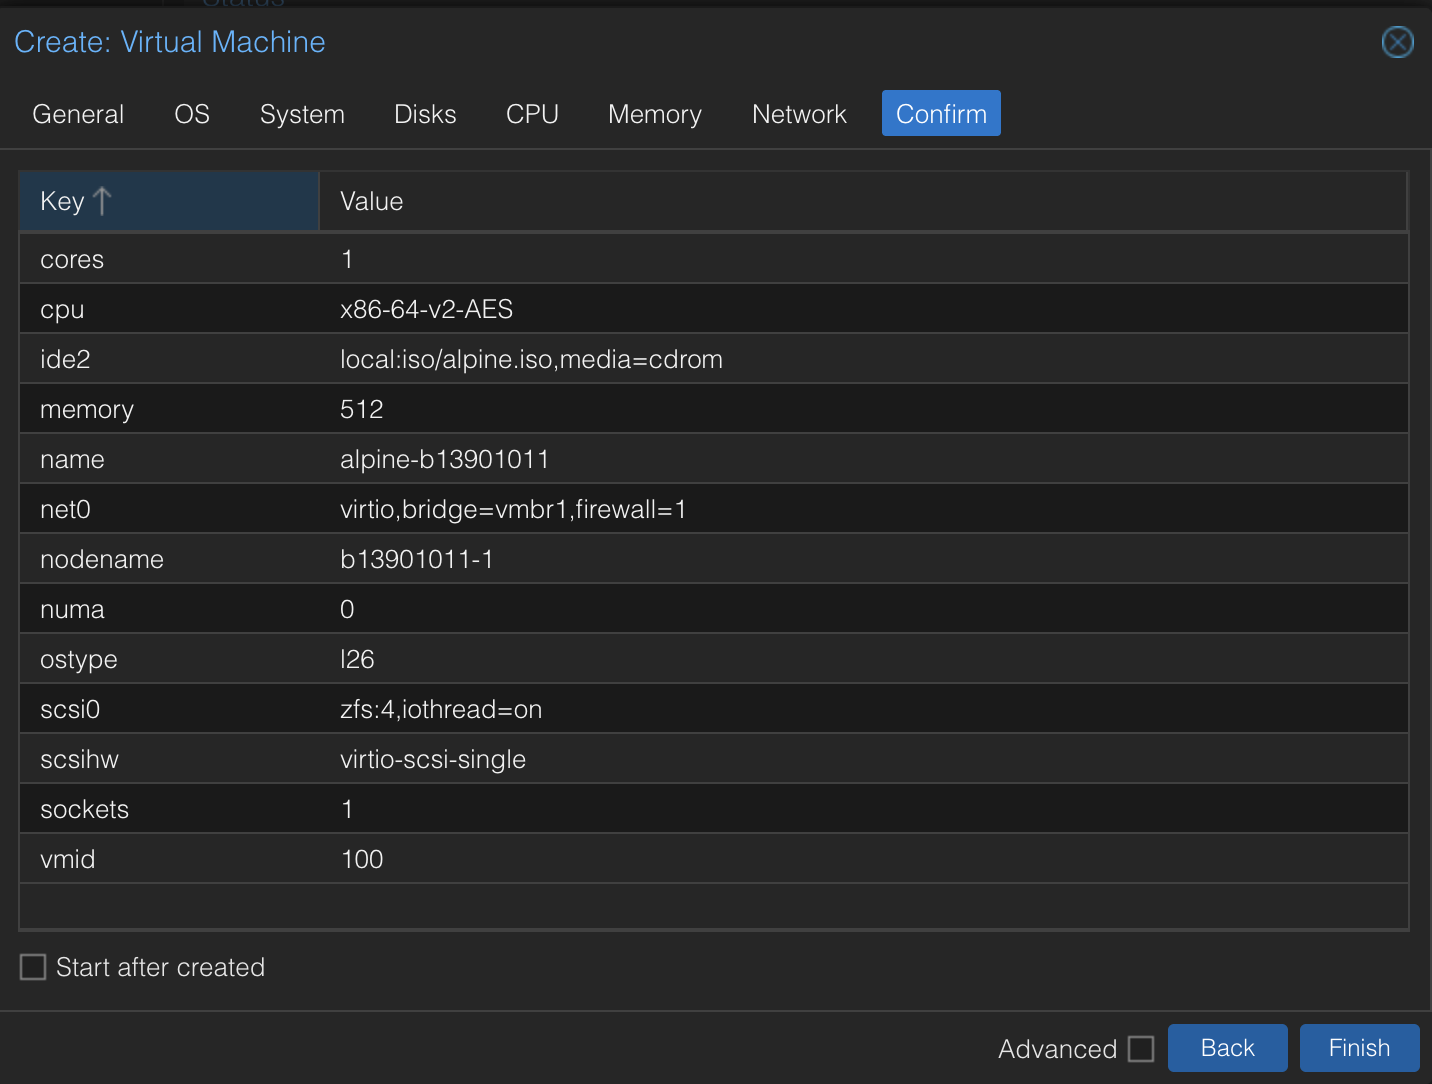
\includegraphics[width=\textwidth]{2-4-5.png}
    \caption{虛擬機器設定}
    \label{fig:2-4-1}
  \end{figure}
  \item 創立完成後，點選 \texttt{Start} ，再點選 \texttt{Console}，並且選擇 \texttt{VNC}，然後點選 \texttt{Connect}，瀏覽器會跳出一個新的分頁，開啟 VNC 連線。
  \item 登入後，執行 \texttt{setup-alpine} ，並且根據以下設定進行安裝：
  \begin{itemize}
    \item Keyboard layout: \texttt{tw} > \texttt{tw}
    \item hostname: \texttt{alpine-b13901011}
    \item network: \texttt{eth0} > \texttt{dhcp} > \texttt{no}
    \item Timezone: \texttt{Asia/Taipei}
    \item APK Mirror: \texttt{35} (nycu)
    \item ssh server: \texttt{openssh}
    \item allow root ssh login: \texttt{yes}
    \item Disk and Install: \texttt{vda} > \texttt{sys}
  \end{itemize}
  \item 安裝完成後，回到 Web UI 頁面關閉虛擬機。
  \item 在 Web UI 頁面中，點選 \texttt{alpine-b13901011} > \texttt{Hardware} > \texttt{CD/DVD Drive (alpine.iso)} > \texttt{Remove}。
  \begin{figure}[H] 
    \centering
    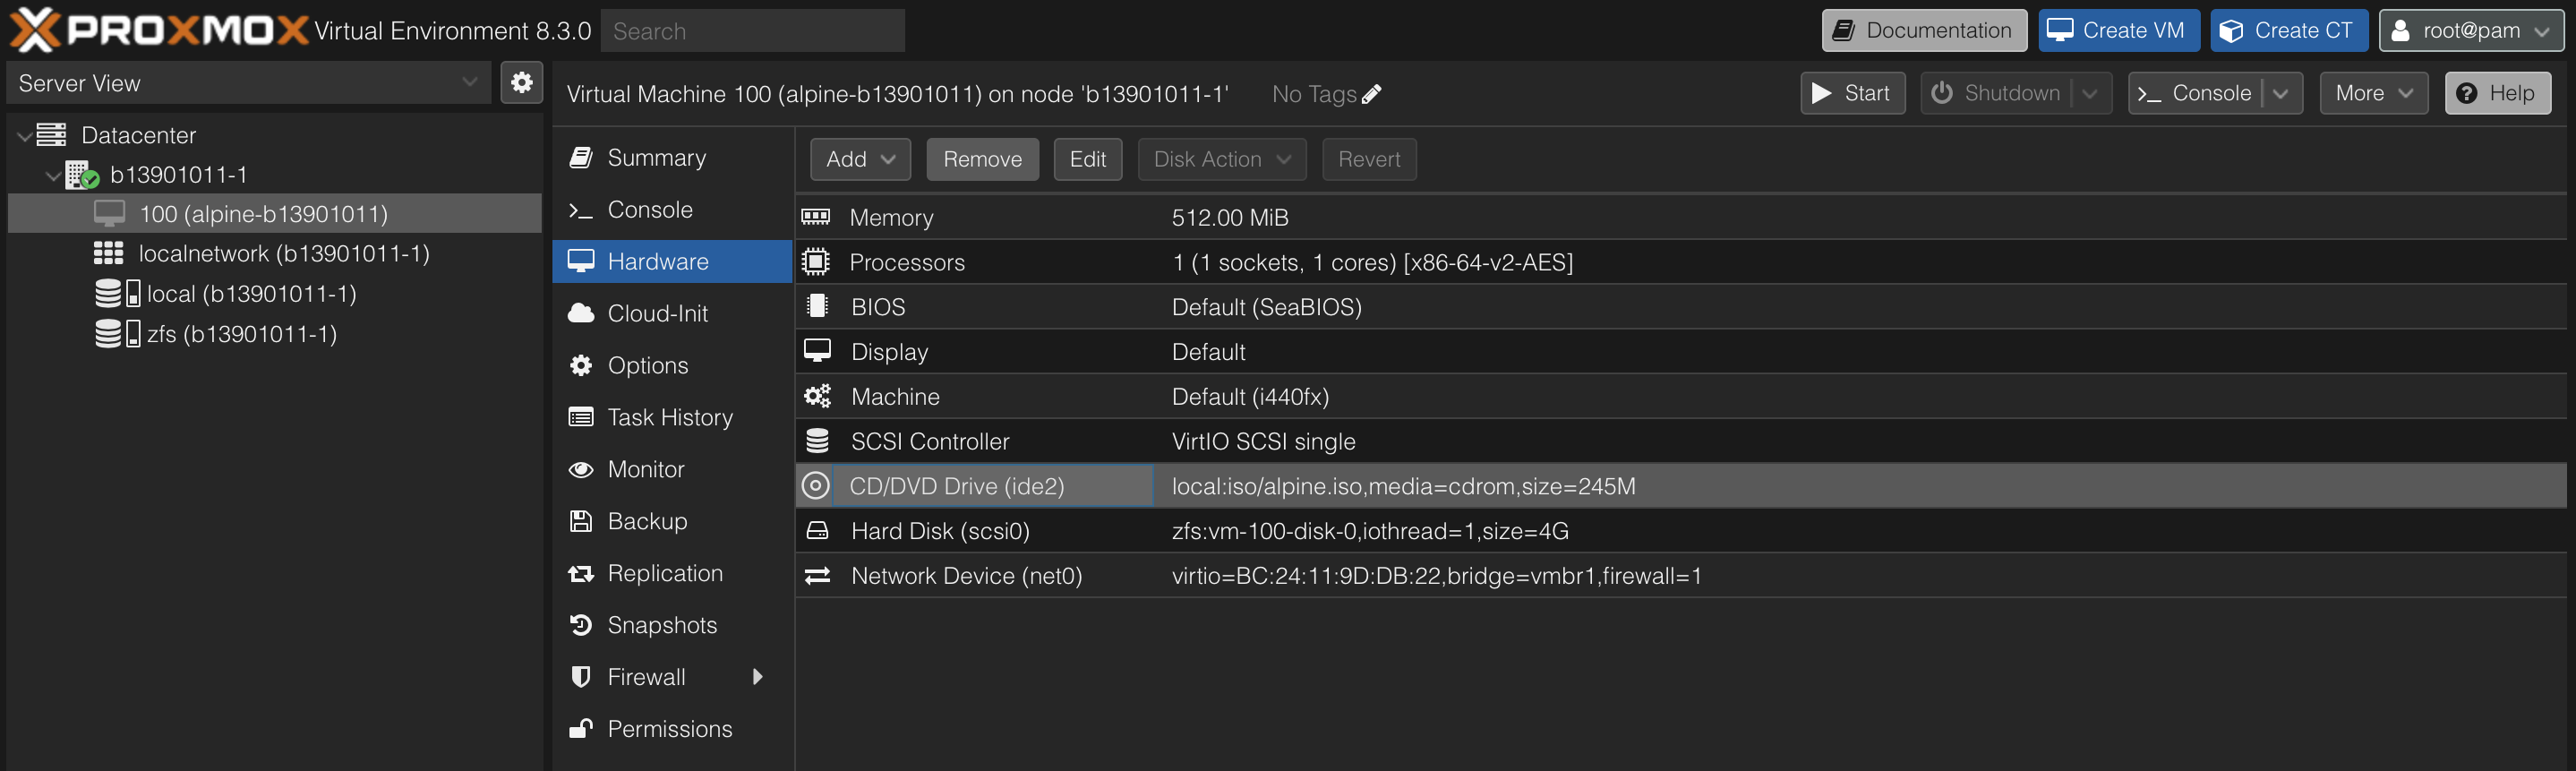
\includegraphics[width=\textwidth]{2-4-6.png}
    \caption{移除 CD/DVD Drive}
    \label{fig:2-4-6}
  \end{figure}
  \item 重新開機後，進入 Console，即完成。
  \begin{figure}[H]
    \centering
    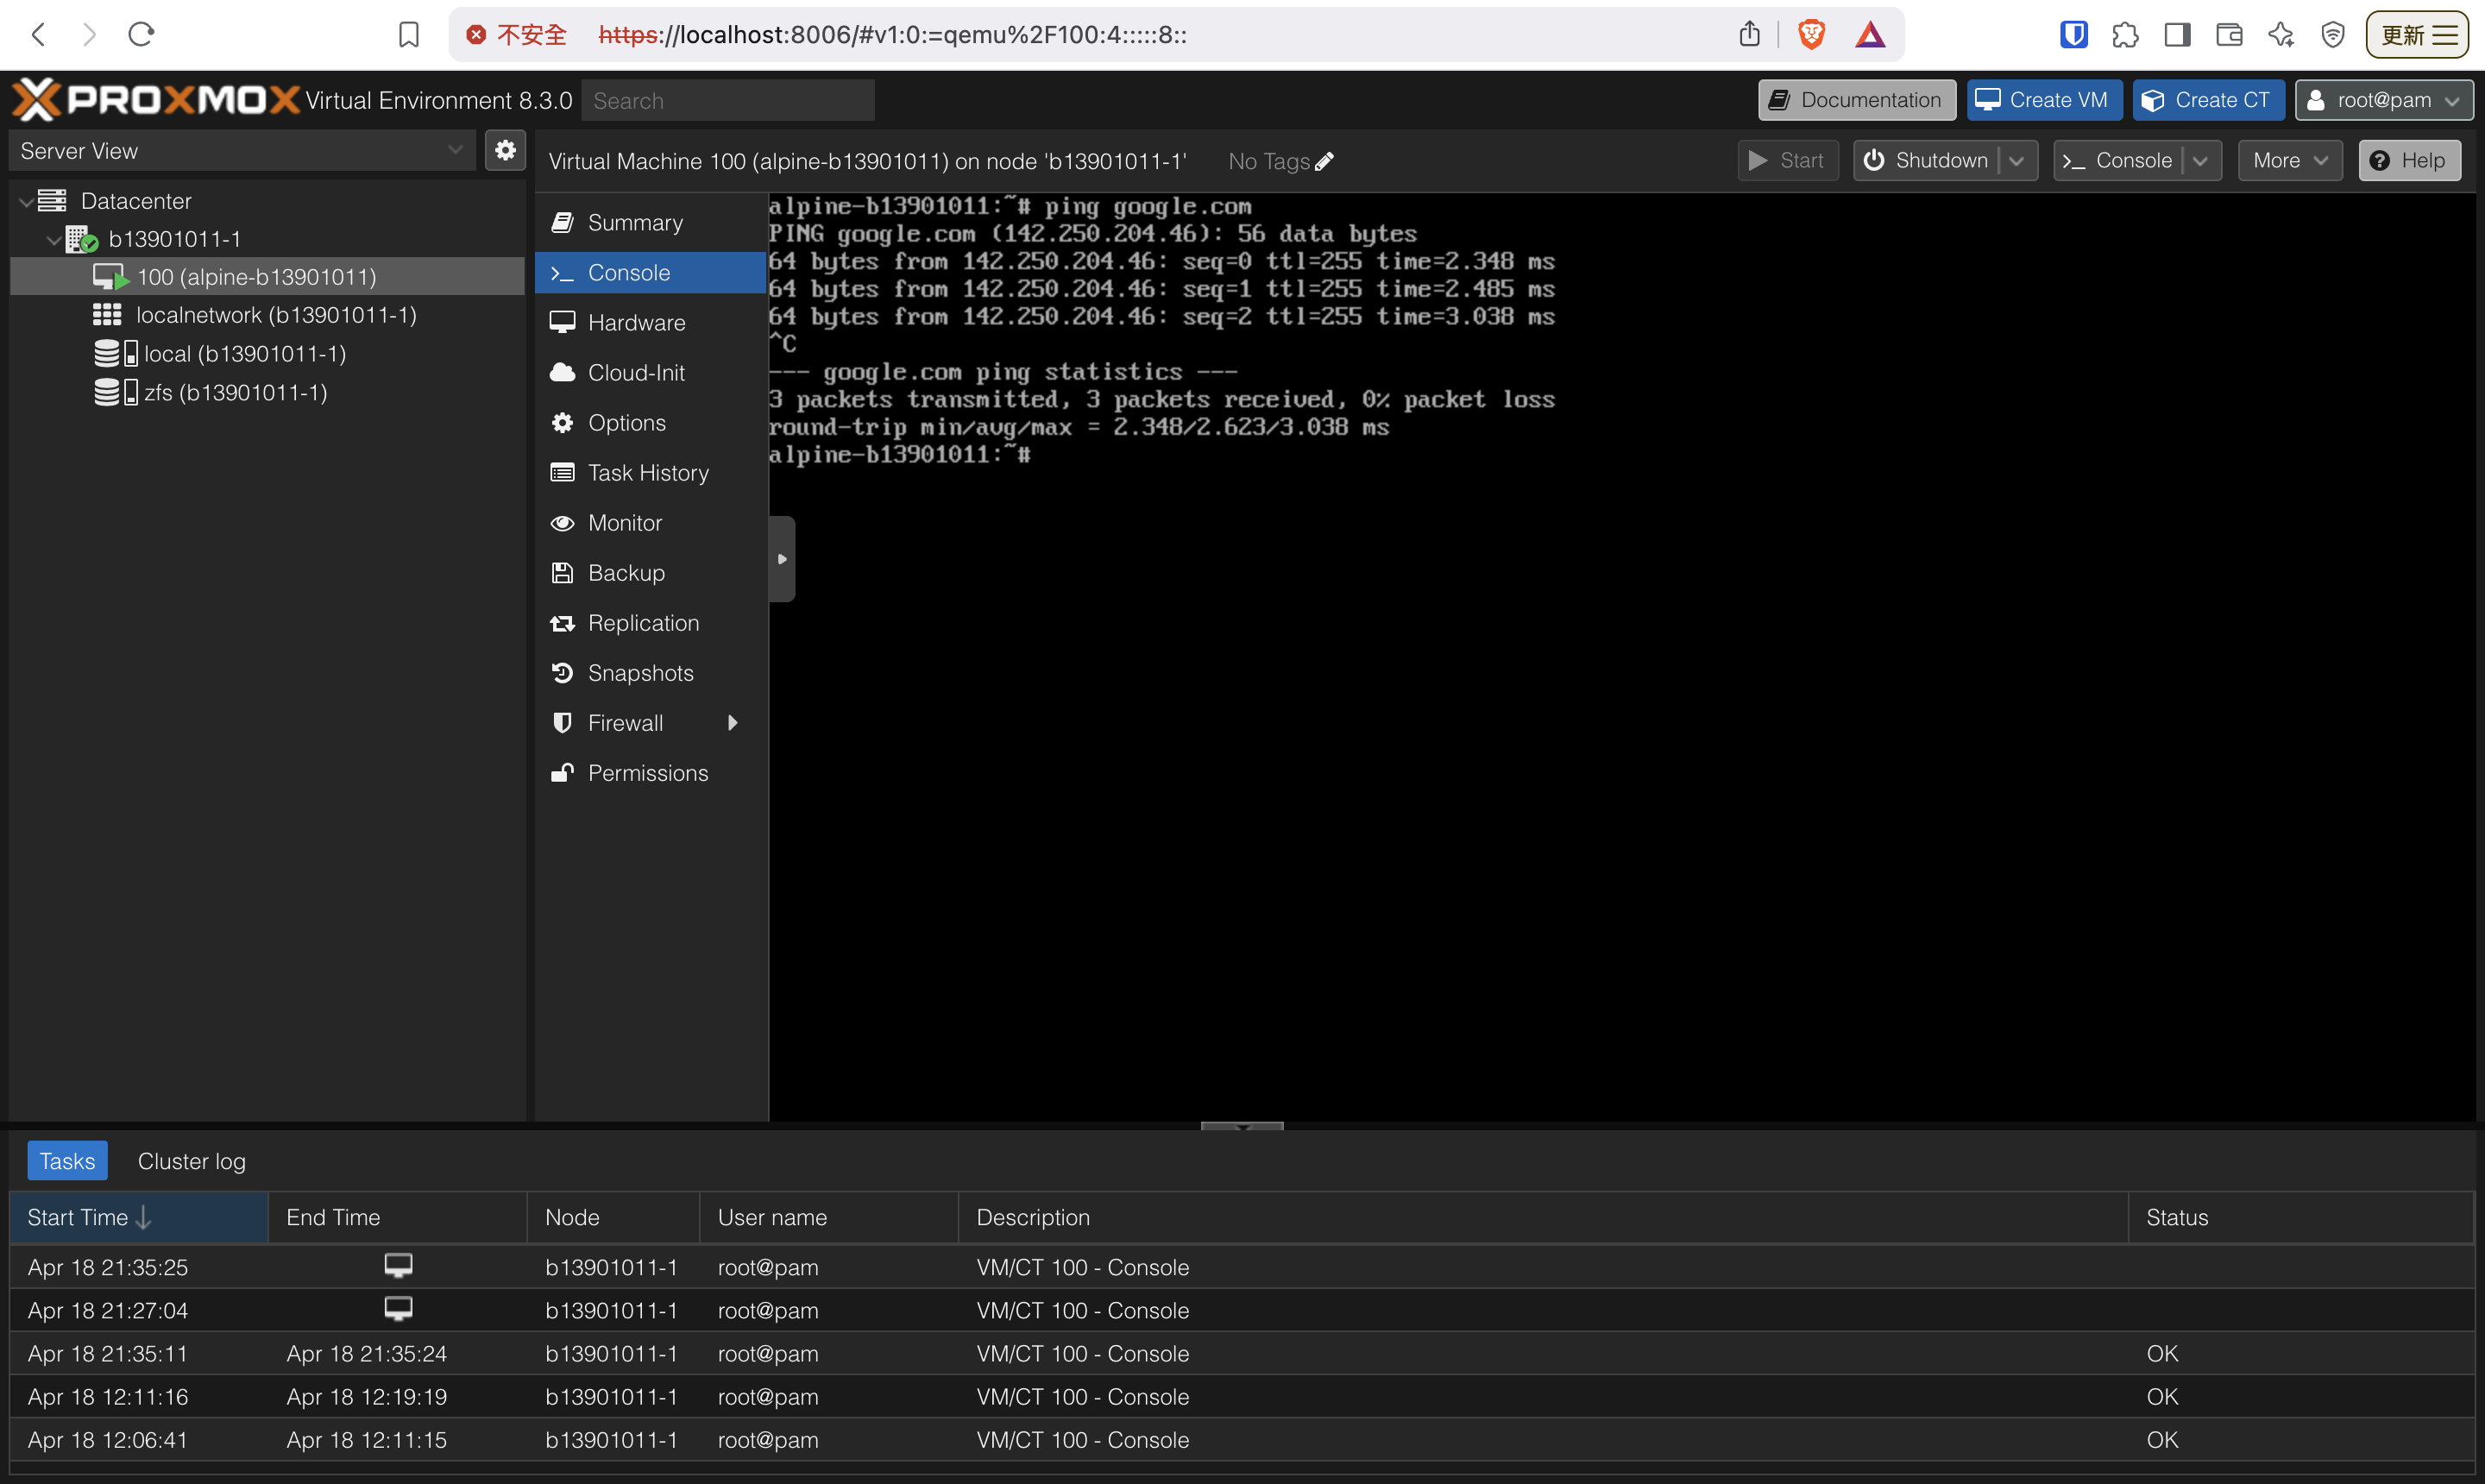
\includegraphics[width=\textwidth]{2-4-7.png}
    \caption{虛擬機器啟動畫面}
    \label{fig:2-4-7}
  \end{figure}
\end{enumerate}


% Problem 2.5
\clearpage
\subsection{}
在虛擬機器中，我使用 \texttt{setup-user} 指令來創建使用者，並且依據指令填入使用者名稱等資訊，如下所示：
\begin{figure}[H]
  \centering
  
\includegraphics[width=\textwidth]{2-5-1.png}
  \caption{創建使用者}
  \label{fig:2-5-1}
\end{figure}
\subsection{}
以下為使用新增的使用者成功登入 alpine 虛擬機的畫面：
\begin{figure}[H]
  \centering
  
\includegraphics[width=\textwidth]{2-5-2.png}
  \caption{以 b13901011 登入}
  \label{fig:2-5-2}
\end{figure}


\clearpage
% -----------------------------------------------------------
% Problem 3
% -----------------------------------------------------------
\section{Cluster and HA}
\begin{mycolorbox}[teal]
  \textbf{Reference:}
  \footnotesize
  \begin{itemize}
    \item 
  \end{itemize}
\end{mycolorbox}

% Problem 3.1
\subsection{}

% Problem 3.2
\subsection{}

% Problem 3.3
\subsection{}

% Problem 3.4
\subsection{}

% Problem 3.5
\subsection{}

% Problem 3.6
\subsection{}

% Problem 3.7
\subsection{}


% -----------------------------------------------------------
%    You don't have to mess with anything below this line.
% -----------------------------------------------------------

\end{document}
